% intro_biographie.tex -- fragment LaTeX (sans préambule). Révision de style du 24 oct. 2026 ; faits, sources et
%   citations du carnet contrôlés sur la transcription définitive.
\section{Hippolyte Combes (1876–1970)}

Quand il ouvre son \textit{Livre-Journal}, le 25~juillet 1916, Hippolyte Combes va avoir quarante ans. Avocat devenu professeur d'anglais, il est depuis plus de quatorze mois interprète auprès de l'armée britannique. Il est fiancé et se mariera l'année suivante. Sa vie est connue par peu de pièces --- acte de naissance, fiche matricule, quelques lettres et cartes, des imprimés --- et par les études de son petit-fils Pierre Combes, qui rapportent les souvenirs de la famille\footnote{P.~Combes, «~Mon grand-père Hippolyte Combes (et ses sœurs)~», texte inédit illustré, s.~d., et \textit{Une étude de la famille Combes de Castelnau-Pégayrols}, texte inédit, version du 19~mars 2023, archives familiales (ci-après : P.~Combes, «~Mon grand-père~», et P.~Combes, \textit{Étude}) ; le premier texte reprend un chapitre du second. L'auteur cite comme sources des registres paroissiaux, sa correspondance avec les archives de l'Aveyron et de Millau, des lettres de famille et les traditions orales de son grand-père.}. On distingue ici ce que les documents établissent, ce que la tradition rend probable et ce qui reste hypothèse.

\subsection{Une famille millavoise}

\begin{figure}[tbp]
\centering
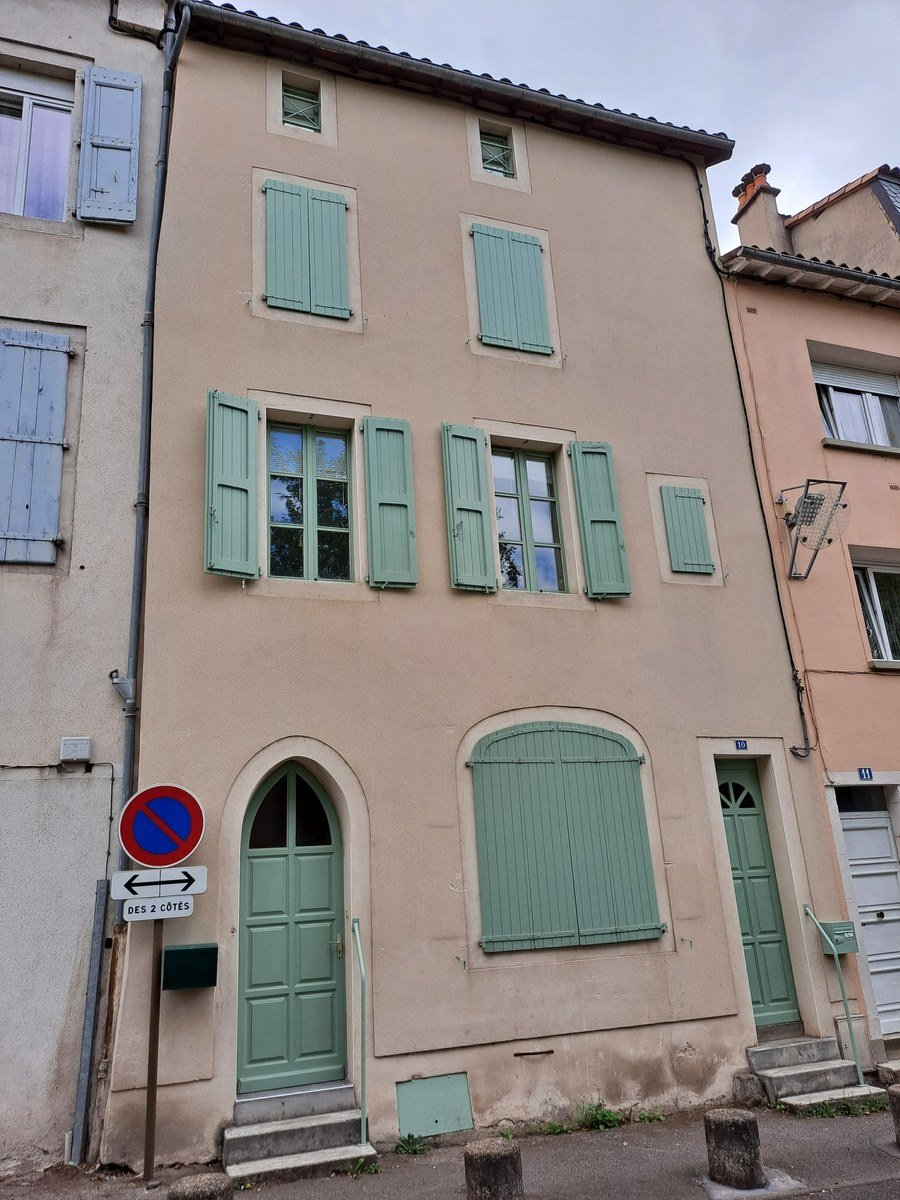
\includegraphics[width=0.62\textwidth,height=0.40\textheight,keepaspectratio]{illustrations/maison_millau.jpg}
\caption{Millau, la maison Combes (photographie récente ; archives familiales).}
\end{figure}


Marie Lucien Hippolyte Combes naquit à Millau le 14~août 1876, à dix heures du soir, d'un avocat de quarante-neuf ans, François Augustin Hippolyte Combes, et de Marie Anaïs Alric. L'acte, dressé le surlendemain, l'emporte sur la fiche matricule, recopiée en 1921, qui donne le 22~août, et sur un arbre familial qui donne le 19\footnote{Acte de naissance n\textsuperscript{o}~395, Millau, 16~août 1876, copie numérique, archives familiales (rue de lecture incertaine : «~rue des T[o]rrilouts~»). Fiche matricule, recrutement de Toulouse, classe 1896, n\textsuperscript{o}~911, établie le 30~novembre 1921, copie numérique, archives familiales (ci-après : fiche matricule ; relevé en annexe, p.~\pageref{annexe-services}). P.~Combes, étude familiale illustrée, version de 2020–2021, archives familiales, p.~52 et 98 (arbres ; ci-après : arbres de 2020).}.

La famille paternelle venait de Castelnau-Pégayrols, près de Millau. Le grand-père, François (1789–1855), entra comme «~garçon menuisier~» chez un oncle établi rue Saint-Martin, à Millau, hérita de la maison et de l'atelier, devint, dit-on, un ébéniste recherché et fit étudier son fils. Celui-ci, Hippolyte~I (1825–1899), fit son droit à Toulouse et y plaida, puis revint à Millau, où il fut inscrit au barreau au moins de 1879 à 1885. Le 22~juillet 1864, à près de quarante ans et après de longues fiançailles, il avait épousé sa cousine Anaïs Alric (1838–1907), fille d'un limonadier millavois\footnote{P.~Combes, \textit{Étude}, chap. «~Les Combes de Millau~» et «~L'avocat Hippolyte Combes~» ; l'arbre de 2020 (p.~52) date le mariage du 20~juillet. L'âge donné au père en 1876 suppose une naissance en 1826 ou 1827 plutôt qu'en 1825.} (fig.~\ref{arbre-combes}). Leurs neuf enfants furent tous prénommés d'abord Marie. Cinq moururent jeunes, de tuberculose selon la tradition, qui accuse l'insalubrité de la rue Saint-Martin. Survécurent Françoise (1871–1942), carmélite à Périgueux sous le nom de sœur Marie de la Croix, qui écrivit souvent à son frère ; Joséphine (1873–1914), qui devait tenir la maison de celui-ci ; Maria (1875–1903), religieuse missionnaire, morte de la typhoïde à Carthage à la fin de son noviciat ; enfin Hippolyte, seul fils survivant, «~particulièrement gâté~» par ses parents et ses sœurs\footnote{P.~Combes, \textit{Étude} (d'après l'état civil de Millau), et «~Mon grand-père~». L'arbre de 2020 (p.~52) décale de deux jours les naissances de Françoise et de Joséphine ; l'état civil, non consulté, tranchera.}.

Selon la tradition, l'enfance se passa surtout à Toulouse, avec des vacances à Millau ; en 1896, les parents habitaient Toulouse, 47, rue du Taur. Hippolyte garda toute sa vie la maison de la rue Saint-Martin, aujourd'hui 10, place Emma-Calvé ; il la louait en s'y réservant une chambre. Elle ne fut vendue qu'après sa mort\footnote{P.~Combes, «~Mon grand-père~», et \textit{Étude} ; fiche matricule.}. En 1897, l'étudiant de vingt et un ans raconta dans un cahier ce qui fut peut-être la dernière visite de Maria à ses parents ; il le dédia «~A ma sœur tendrement affectionnée Joséphine~», avec en épigraphe la phrase de Sénèque «~Les grandes douleurs sont muettes~». Dans une lettre que la tradition ne date pas, le père d'Adhémar, jésuite et «~grand ami des Combes~», reprochait au jeune homme, «~alors agnostique~», d'accroître par ses sarcasmes contre cette vocation la douleur de sa mère et de sa sœur Françoise\footnote{P.~Combes, «~Mon grand-père~», qui cite le cahier et la lettre ; ces pièces n'ont pas été vues. Le «~père d'Adhémar~» est très probablement Alfred d'Adhémar de Cransac, «~le Supérieur~» des jésuites de Toulouse selon la presse de 1912, mort le 16~septembre 1914 à soixante-seize ans (\textit{Le Télégramme}, 23~novembre 1912, p.~3 ; faire-part, \textit{L'Express du Midi}, 18~septembre 1914, p.~2).}.

\subsection{Le droit, l'Angleterre, l'enseignement}

\begin{figure}[tbp]
\centering
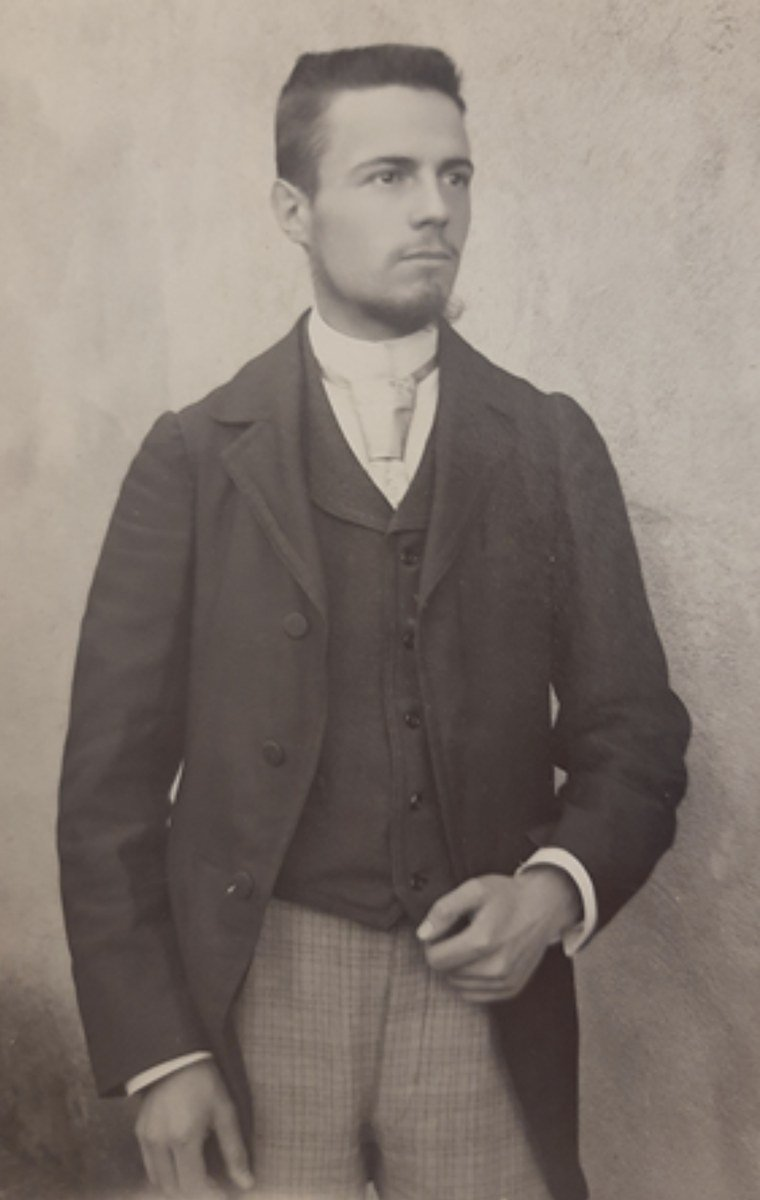
\includegraphics[width=0.5\textwidth,height=0.40\textheight,keepaspectratio]{illustrations/hippolyte_1897.jpg}
\caption{Hippolyte Combes à vingt et un ans, en 1897 (archives familiales).}
\end{figure}


Hippolyte étudia à Toulouse, au petit séminaire de l'Esquile, au lycée, puis à la faculté\footnote{P.~Combes, «~Mon grand-père~».}. Recensé avec la classe 1896 comme «~étudiant en droit~» (1,66~m, cheveux bruns, yeux châtains), il fut «~exempté après ajournement de deux ans~» pour «~faiblesse générale~»\footnote{Fiche matricule.}. Selon la tradition, sa mauvaise vue lui fit renoncer à la marine ; le carnet montre du moins qu'il portait un lorgnon, qu'il fait réparer puis remplacer (ff.~4~v\textsuperscript{o}, 56~v\textsuperscript{o} et 61~r\textsuperscript{o})\footnote{P.~Combes, «~Mon grand-père~», et courriel de Pierre Combes, 11~octobre 2021, archives familiales.}. La tradition et l'éloge prononcé à l'Académie de Montauban en 1938, deux sources indépendantes, s'accordent sur l'essentiel : licencié en droit et avocat, il passa ensuite une licence d'anglais. Selon l'éloge, il plaida quelque temps à Toulouse puis, «~ayant sa licence d'anglais, et désirant abandonner sa profession d'avocat~», demanda une chaire d'anglais\footnote{Discours de réception d'Henri Pouvillon, 7~février 1938, \textit{Recueil de l'Académie de Montauban}, 2\textsuperscript{e}~série, t.~XLVIII, année 1938, Montauban, Forestié, 1939, p.~150 (l'éloge passe directement du barreau au lycée de Montauban) ; P.~Combes, «~Mon grand-père~».}.

Pour la décennie suivante, on n'a que la tradition. À la mort de son père, le 11~août 1899, il serait entré aux chemins de fer pour faire vivre sa mère et Joséphine, jusqu'à devenir sous-chef de gare à Brive-la-Gaillarde. Puis il aurait démissionné et vécu quatre ans en Angleterre, notamment à Nottingham, de leçons de français et de la vente de fleurs, en photographiant beaucoup. Il serait rentré en 1907, à la mort de sa mère\footnote{P.~Combes, «~Mon grand-père~» : «~La photo était son violon d'Ingres~».}. Aucune pièce ne confirme ce séjour, mais il s'accorde avec la maîtrise de l'anglais qu'attestent sa carrière et son carnet, et avec une carte de 1918 où il dit se plaire dans une église normande «~autant que dans les plus belles cathédrales de France et d'Angleterre~»\footnote{Carte à Marguerite Combes, Les Andelys, 28~novembre 1918, archives familiales.}.

La tradition lui prête ensuite des postes à Corte et à Blaye, avant Nogent-le-Rotrou ; Joséphine, cardiaque, le suivait et tenait sa maison. Seul Nogent est documenté : il se dit «~prof. au coll. de Nogent-le-R.~» au bas d'une minute de lettre, le conseil de révision d'Eure-et-Loir le reclasse en 1914, et sa nomination à Montauban est publiée en 1919 au nom de «~M.~Combes (Nogent-le-Rotrou)~»\footnote{Minute autographe d'une supplique sur l'indemnité des interprètes, s.~d., archives familiales (mention biffée) ; fiche matricule ; \textit{Les Langues modernes}, 17\textsuperscript{e}~année, 1919, n\textsuperscript{o}~3, «~Chronique du mois~», p.~184. Corte et Blaye ne reposent que sur P.~Combes, «~Mon grand-père~».}. Il habitait au 47 (ou 17), rue Saint-Hilaire, une maison qui avait, écrira-t-il, «~un petit air flamand~». Pendant la guerre, il garda ce «~chez moi du Perche~» et son appartement de la rue de Languedoc, à Toulouse : en août 1916, il expédie un sac de linge à Nogent (f.~12~r\textsuperscript{o}–v\textsuperscript{o}) ; en octobre, il paie à Toulouse un «~Semestre~» de 90~F, sans doute son loyer (f.~31~r\textsuperscript{o})\footnote{Carte à Marguerite Combes, Paris, 25~novembre 1918, archives familiales. Le numéro est de lecture incertaine, sur cette carte comme sur la fiche matricule.}. La même carte rappelle des séjours à Paris, à lire dans la grande salle de la bibliothèque Sainte-Geneviève : «~Que de fois Joséphine m'y a-t-elle accompagné ! Elle lisait à côté de moi.~»\footnote{\textit{Ibid.} La date et l'objet de ces séjours sont inconnus ; la préparation d'un concours est une hypothèse.} Il n'était pas agrégé : il sera nommé à Montauban, en 1919, comme «~chargé de cours~». Plus tard, marié et père de famille, il échoua, selon la tradition, à l'agrégation d'anglais «~à Bordeaux~»\footnote{P.~Combes, «~Mon grand-père~» ; \textit{Les Langues modernes}, \textit{loc.~cit.} Hippolyte Combes dit avoir assisté «~en curieux~» à une soutenance de thèse à la faculté des lettres de Bordeaux (\textit{Recueil de l'Académie de Montauban}, année 1932, p.~47).}.

La guerre trouva le frère et la sœur à Nogent. Selon la tradition, Joséphine y mourut d'une crise cardiaque en octobre 1914, à quarante et un ans ; elle voulut être ensevelie avec la photographie du père d'Adhémar épinglée sur sa robe, et son corps fut ramené dans le caveau familial de Millau\footnote{P.~Combes, «~Mon grand-père~» ; arbres de 2020, p.~52. Aucun acte de décès n'a été vu : l'état civil de Nogent-le-Rotrou (Archives départementales d'Eure-et-Loir) et les transcriptions de Millau restent à consulter.}. Le carnet donne un terme : le 30~septembre 1916, Hippolyte Combes associe sa sœur à un ami défunt dans un même «~souvenir~» (f.~29~r\textsuperscript{o}) ; elle était donc morte à cette date. Si l'on retient octobre 1914, que rien ne contredit, la lettre du 16~juin 1916, que la famille croyait adressée à Joséphine, s'adresse plutôt à la carmélite Françoise, seule sœur alors vivante et correspondante régulière de son frère\footnote{Lettre d'Hippolyte Combes, «~Au front, vendredi 16~juin 1916~», 4~p., archives familiales, commençant par «~Ma très chère Sœur~» ; certaines formules («~Que cela dure ainsi. Amen !~») conviennent à une religieuse.}.

\subsection{De l'artillerie à l'armée britannique}

\begin{figure}[tbp]
\centering
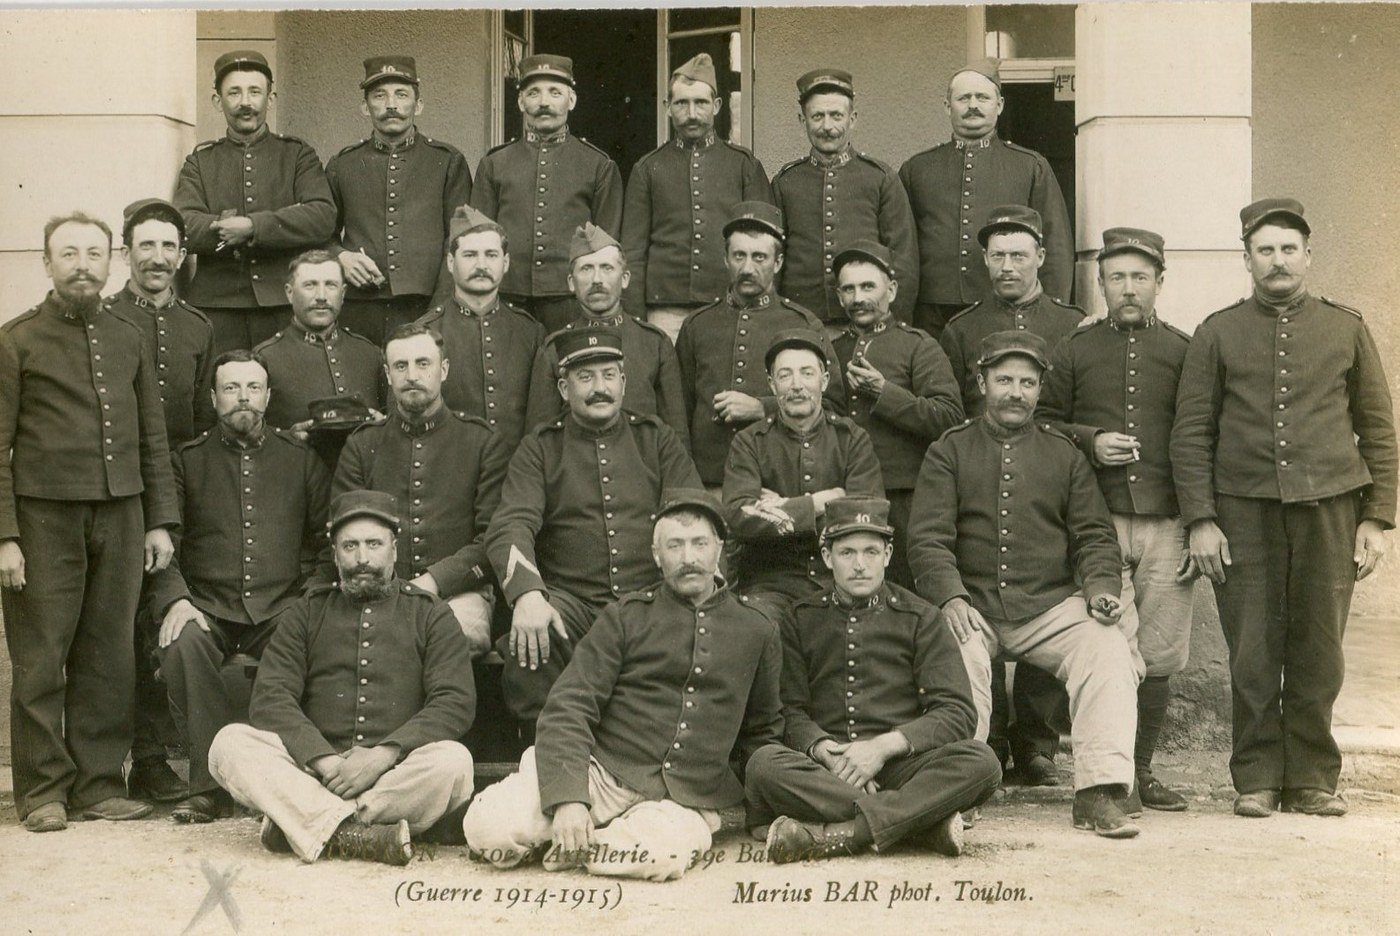
\includegraphics[width=\textwidth,height=0.40\textheight,keepaspectratio]{illustrations/toulon_artillerie_1915.jpg}
\caption{Hippolyte Combes et ses camarades canonniers à l'école d'artillerie de Toulon, avril 1915 (archives familiales).}
\end{figure}


Exempté, Hippolyte Combes ne fut pas mobilisé en août 1914, contrairement à ce que dit la tradition. Le 18~décembre 1914, en application du décret du 9~septembre sur la révision des exemptés, le conseil de révision d'Eure-et-Loir le classa dans le service armé. Rappelé le 20~mars 1915, il arriva le lendemain «~au 10\textsuperscript{e} artillerie~», à Toulon ; une photographie de groupe, datée par la famille d'avril 1915, le montre parmi les canonniers de la 39\textsuperscript{e}~batterie\footnote{Fiche matricule ; photographie de Marius Bar, photographe à Toulon, légendée «~Toulon --- 10\textsuperscript{e} d'Artillerie. - 39\textsuperscript{e} Batterie~» et «~(Guerre 1914-1915)~», archives familiales. P.~Combes, «~Mon grand-père~», place le rappel à la mobilisation générale.}. Il intitule cette instruction «~Six Semaines (de bagne) à Toulon~» dans le plan de ses \textit{Feuillets de Route} (annexe, p.~\pageref{annexe:doc6}, chap.~\textsc{ii} ; cf. f.~62~r\textsuperscript{o}, où M.~Renard, à Auxi-le-Château, lui montre un coffret «~acheté en 1858 au bagne de Toulon~»). Le métier ne lui convenant pas, il réussit l'examen d'interprète. Le 4~mai 1915, il partit aux armées, «~détaché à la Mission militaire française attachée à l'armée britannique comme interprète~»\footnote{Fiche matricule ; P.~Combes, «~Mon grand-père~». Sur le recrutement et le statut des interprètes, voir la section suivante.}.

Selon la tradition familiale, il fut d'abord affecté, en mai 1915, au 1st Battalion, Irish Guards, et y approcha le prince de Galles, le futur Édouard~\textsc{viii}. Une petite-fille, Danièle Boyer, écrit : «~il était un des interprètes du prince de galles. c'est ce que disait mon grand-père quand j'étais petite~»\footnote{Courriel de Danièle Boyer, 7~décembre 2025 ; P.~Combes, «~Mon grand-père~», et message du 26~novembre 2025 ; archives familiales.}. Le plan autographe des \textit{Feuillets de Route} (annexe, p.~\pageref{annexe:doc6}) confirme le service aux Irish Guards. Après «~III - Départ pour le front~» et «~IV - A la base anglaise de Rouen~» --- grande base britannique et dépôt général de l'\textit{Army Service Corps}, par où passaient les interprètes ---, il y inscrit : «~V - Avec les 1\textsuperscript{st} Irish. Guards~» et «~VI - La veille d'une g\textsuperscript{de} attaque (Mai 1915)~». Le rôle auprès du prince reste une tradition. En mai 1915, le bataillon, alors dans la 4th Guards Brigade de la 2nd Division, prit part à l'offensive de Festubert (15–25~mai 1915) ; en juin et juillet, il tint le secteur de Cuinchy et de Cambrin, avec ses cantonnements de repos à Béthune et à La Couture. Le prince de Galles, officier à l'état-major du I~Corps à Béthune, lui rendit plusieurs visites avant de rejoindre la Guards Division, formée près de Saint-Omer en août 1915\footnote{R.~Kipling, \textit{The Irish Guards in the Great War}, t.~I, Londres, Macmillan, 1923, sections «~The Battle of Festubert~» et «~From Festubert to Loos~», p.~63–95. Le journal de marche dont les archives familiales ont une copie (TNA, WO~95/1216/1) couvre le 1st Battalion, Irish Guards, dans la 1st Guards Brigade, d'août 1915 à janvier 1919, après le départ d'Hippolyte Combes ; mai–juillet 1915 relève de la 2nd Division (WO~95/1343/3).}. Le \textit{Livre-Journal} renvoie à ce séjour en Artois : Hippolyte Combes compare la Grand-Place de Béthune à celle de Bailleul (f.~4~r\textsuperscript{o}, 1\textsuperscript{er}~août 1916), et il y avait connu l'interprète Cordonnier, retrouvé le 4~novembre 1916 à Bertrancourt (f.~46~v\textsuperscript{o} : «~retrouvé interprète Cordonnier, R.F.A –, que connu à Bethune~»).

Sa lettre du 25~février 1916 (annexe, p.~\pageref{annexe:doc1}) et les chapitres \textsc{vii} à \textsc{ix} du plan des \textit{Feuillets de Route} permettent de suivre l'été et l'automne 1915. À Saint-Omer, siège du grand quartier général britannique et de la Mission militaire française, le retrouva un ancien camarade de la faculté de Toulouse devenu capitaine. À la fin de juillet, il fut «~attaché à la 18\textsuperscript{e} division qui se formait dans les parages de Flesselles~». Secrétaire du bureau divisionnaire de la Mission française, il se lassa en quinze jours de «~cette vie trop sédentaire et monotone~» et obtint, en août, d'être affecté à une compagnie du train divisionnaire de l'\textit{Army Service Corps} (\textit{«~VII - Un train d'A.S.C. — Le ventre d'1 brigade / Avec l'A.S.C.~»})\footnote{Copie autographe d'une lettre à un capitaine, «~Au front~», 25~février 1916, annexe, p.~\pageref{annexe:doc1} ; plan des \textit{Feuillets de Route}, annexe, p.~\pageref{annexe:doc6}. Sur la concentration de la division près de Flesselles, voir p.~\pageref{intro:division}.}. À la fin de l'été 1915, il connut avec cette unité les cantonnements dans les bois entre l'Ancre et la Somme (\textit{«~VIII - Villégiature estivale dans les bois~»}, autour de Bray-sur-Somme, Suzanne, Fricourt, Méricourt-l'Abbé et Ribemont-sur-Ancre ; cf. f.~76~v\textsuperscript{o}) et l'incident de cantonnement de Morlancourt (annexe, p.~\pageref{annexe:doc2}), puis la revue du 25~octobre 1915 près de Ribemont-sur-Ancre (\textit{«~IX - Revue d'une division anglaise par le Roi G. et le Prés.\textsuperscript{t} R.\textsuperscript{e} F.\textsuperscript{se}~»} ; voir p.~\pageref{intro:revue}). Dans sa lettre de février 1916, il s'informe aussi d'un «~concours pour être nommé stagiaire~» (voir la section suivante).

Simple soldat, rattaché pour l'administration au train des équipages (voir p.~\pageref{intro:statut}), il appartenait sans doute depuis le 1\textsuperscript{er}~novembre 1916, par son âge, à la réserve de l'armée territoriale\footnote{Fiche matricule, dont la grille des dates de passage n'est interprétée qu'avec réserve ; il écrit en 1918 : «~En majorité nous sommes des territoriaux ou de la R.A.T.~» (carte à Marguerite Combes, Les Andelys, 28~novembre 1918).}. La compagnie de l'\textit{Army Service Corps} qu'il rejoignit en août 1915 est la 152nd Company du carnet, l'une des quatre compagnies hippomobiles du train de la 18th (Eastern) Division, qui ravitaillait la 54th Brigade («~le ventre d'1 brigade~»). Il en fut l'interprète jusqu'au 1\textsuperscript{er}~novembre 1916, puis fut détaché aux achats de paille et de foin de la Fifth Army, à Acheux puis à Hérissart (voir la section suivante). De mai 1917 à l'armistice, son activité n'est pas documentée : la fiche matricule le compte seulement «~aux armées~», en campagne double, jusqu'au 11~novembre 1918.

\subsection{Les fiançailles du carnet}

Marguerite Calmels était née à Millau le 15~avril 1892, fille de Gabriel Calmels (1852–1921), médecin, et de Valentine Cartairade ; l'acte a pour témoin Émile Crouzet, alors agent de change à Millau, mari d'une sœur du médecin (fig.~\ref{arbre-calmels})\footnote{Acte de naissance de Marie Marguerite Calmels, Millau, 16~avril 1892, copie numérique, archives familiales ; P.~Combes, \textit{Étude}, annexe~2, «~Les Calmels~» ; faire-part d'Émile Crouzet, \textit{L'Express du Midi}, 23~décembre 1926, p.~5, émanant notamment de «~Madame Émile Crouzet, née Calmels~». La presse date de décembre 1926 la mort d'Émile Crouzet, que la tradition place en 1921.}. Selon la tradition, ce fut un «~mariage de proposition~», arrangé par la famille Crouzet, «~parente aux Calmels et amie des Combes~», et rendu possible par la mort de Joséphine, qui laissait Hippolyte seul. Lui racontait qu'invité le même jour à Millau, «~vers 1915~», à trois dîners où l'on devait lui présenter une jeune fille, il avait choisi celui des Calmels et des Crouzet. Les deux «~fiancés~» s'écrivirent ensuite\footnote{P.~Combes, «~Mon grand-père~» : «~Libéré par la mort de Joséphine, il put penser à se marier~».}.

Quand s'ouvre le carnet, l'engagement est pris. La première entrée note qu'il a «~pensé très vivement à Margte~» (f.~1~r\textsuperscript{o}). Le 13~août, veille de ses quarante ans, dont le carnet ne dit rien, il a «~attendu en vain un mot~» d'elle (f.~10~r\textsuperscript{o}). La permission d'automne réunit les fiancés à Toulouse, du 27~septembre au 4~octobre 1916 ; Marguerite et sa mère logent chez les Crouzet, à Sainte-Marie-des-Champs, sur la Côte-Pavée. Le mot «~fiancée~» apparaît le 28 (f.~28~r\textsuperscript{o}). Le 29, aux ruines de Purpan, ce sont de «~doux épanchts \& baisers intimes av. ma Femme~», et il achète chez le bijoutier Pfister un sautoir en or, sans doute pour elle (f.~28~v\textsuperscript{o}). Le 30, au cimetière de Terre-Cabade, devant le caveau des jésuites et celui du père Marie-Antoine : «~Margte \& moi, echangé serments profondt émus au souvenir de notre gd ami \& de Josèphe~» (f.~29~r\textsuperscript{o}) ; le «~grand ami~» est très probablement le père d'Adhémar. Le 3~octobre, il présente «~ma Fiancée~» à Mme de Labarthe, «~gde amie affectueuse \& attachée~» (ff.~28~v\textsuperscript{o} et 30~v\textsuperscript{o})\footnote{Sans doute la mère du «~docteur de L.~---~» de la lettre du 16~juin 1916, «~dont la mère m'est tant dévouée~».}. Au départ, Marguerite veut l'accompagner à la gare, et il faut se séparer «~par ménagement pour l'oncle~» (f.~31~v\textsuperscript{o}).

L'hiver apporte une crise que la tradition ignore. Le 22~décembre, une lettre de Marguerite, datée du 17, le laisse «~Très affecte Regrets pour le passe \& appréhensions pour l'avenir~» ; le 24, il note des «~Velléités de rupture~» (f.~56~v\textsuperscript{o}). À Noël : «~Pires pensées traversent mon esprit. Ne puis oublier. Cruelle perplexité~» ; le soir, il retrouve le «~calme d'esprit \& parfait équilibre~» (f.~57~r\textsuperscript{o}). Le contenu de la lettre est inconnu ; la seconde permission semble effacer l'épisode. Le 28~janvier 1917, «~Margte, sur la porte, m'attendait Accueil infiniment tendre~» ; «~Mes sentiments à son égard, douceur infinie~» (f.~66~v\textsuperscript{o}). Le 2~février, il se résout à regret à sacrifier «~3 jours entiers~» de Toulouse (f.~69~r\textsuperscript{o}) pour l'accompagner à Millau, où, le lendemain, les parents de Marguerite lui font «~accueil très affectueux~» (f.~69~v\textsuperscript{o}). «~Elle m'a joué qq morceaux et chanté 1 peu~», note-t-il le lendemain (f.~71~r\textsuperscript{o}). Le 5, tous deux vont «~seuls~» au cimetière, où reposent les parents et la sœur d'Hippolyte, et les adieux sont «~dechirants~» (f.~71~v\textsuperscript{o}). Ensuite, le carnet ne nomme plus Marguerite jusqu'au 30~avril.

\subsection{Mariage et démobilisation (1917–1919)}

Le mariage eut lieu à Millau le 25~octobre 1917, pendant une permission : le menu du repas donne la date, et une photographie montre Hippolyte en uniforme auprès de sa femme\footnote{«~Menu --- 25~octobre 1917~» et photographie de mariage, archives familiales. L'acte de mariage n'a pas été consulté.}. La tradition ajoute que l'abbé Alric les bénit en l'église du Sacré-Cœur, ce qui mit fin à la brouille avec la famille maternelle (aux obsèques de son père, en 1899, Hippolyte avait éconduit un oncle Alric venu faire la paix) ; que le repas fut servi au premier étage de la maison bâtie par le docteur Calmels, 10, rue Alfred-Guibert ; que les époux passèrent leur première nuit rue Saint-Martin et que le mari repartit dès le lendemain pour le front, Marguerite l'accompagnant peut-être jusqu'à Amiens\footnote{P.~Combes, «~Mon grand-père~» et \textit{Étude} ; la tradition mentionne aussi une dot de 50\,000~F.}. Une fille, Valentine, naquit à Millau le 17~septembre 1918 ; son grand-père l'accoucha\footnote{Fichier des personnes décédées de l'INSEE, interrogé par \url{https://deces.matchid.io} le 18~octobre 2026 ; la tradition donne le 18 ou le 19~septembre (P.~Combes, «~Mon grand-père~» ; arbres de 2020, p.~98).}.

\begin{figure}[tbp]
\centering
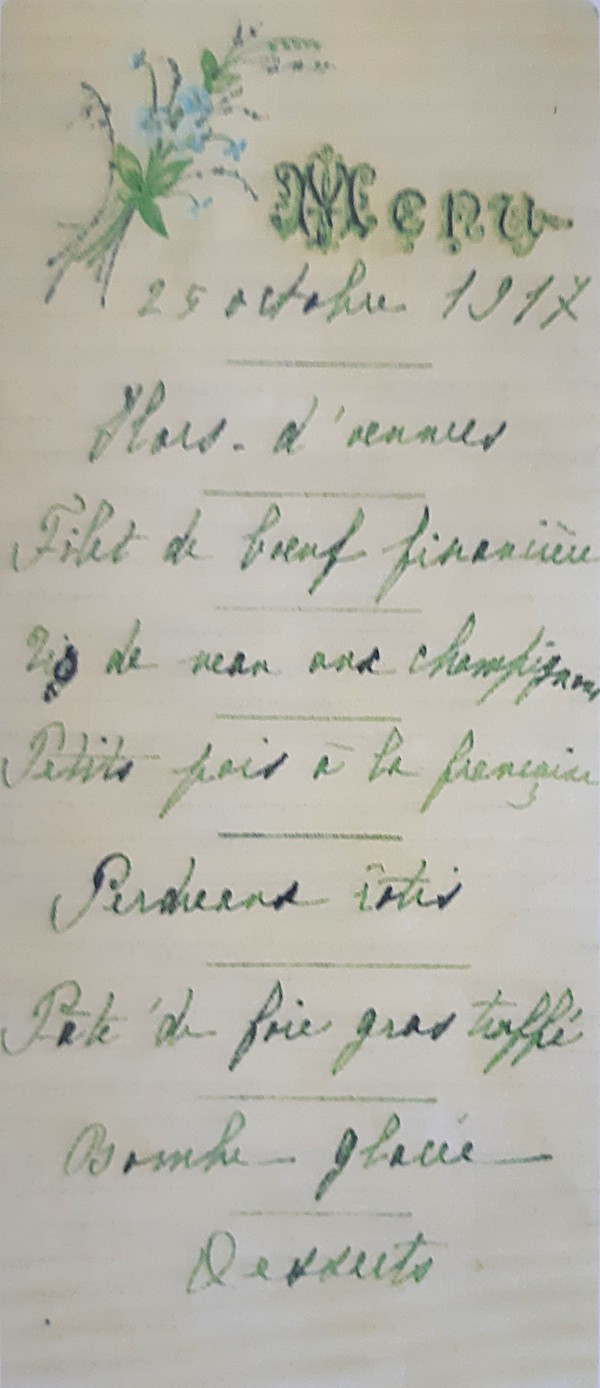
\includegraphics[width=0.48\textwidth,height=0.36\textheight,keepaspectratio]{illustrations/menu_mariage_1917.jpg}\hfill
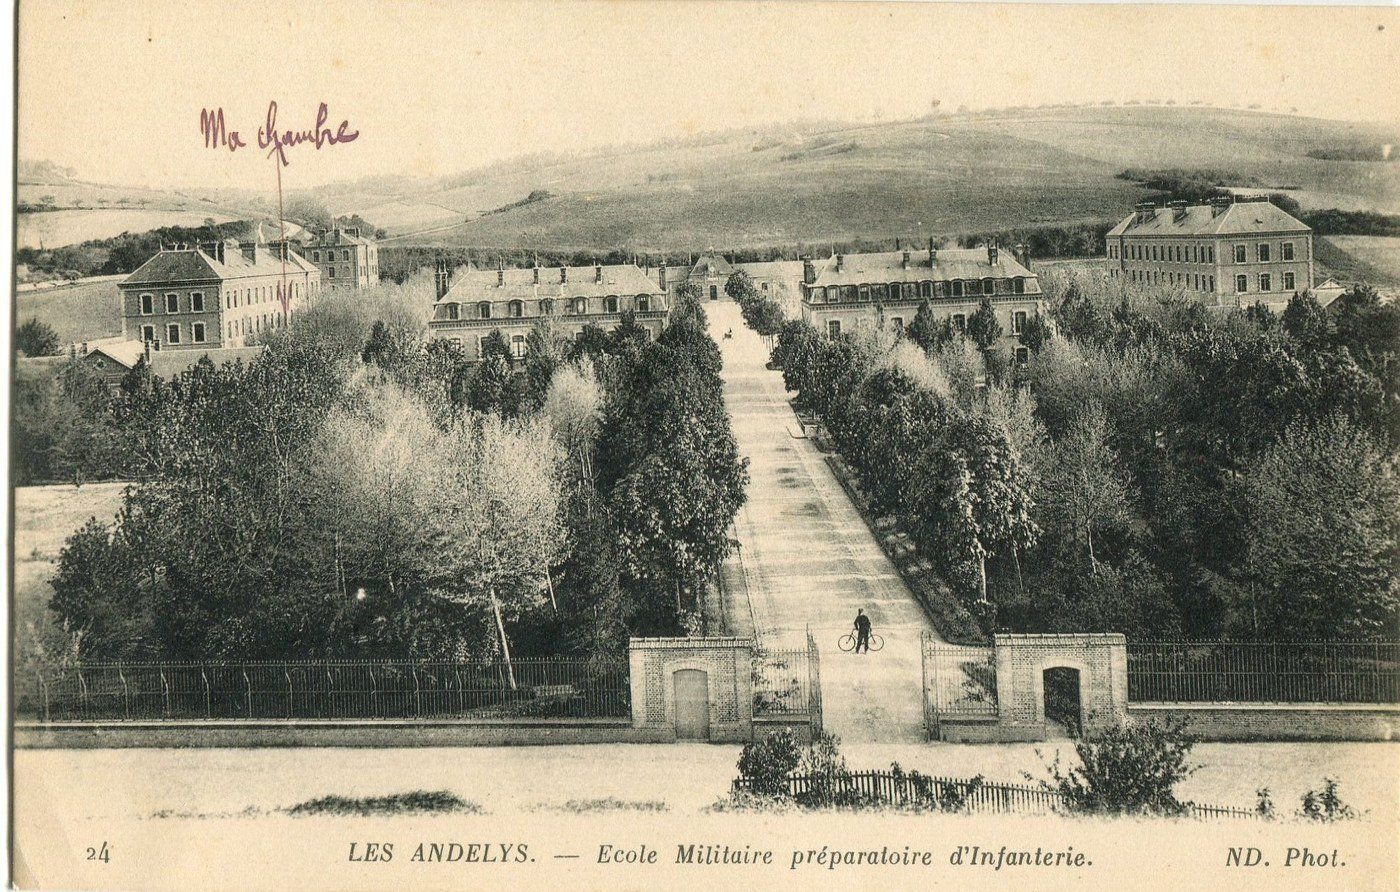
\includegraphics[width=0.48\textwidth,height=0.36\textheight,keepaspectratio]{illustrations/andelys_ecole_militaire.jpg}
\caption{À gauche, le menu du repas de noces, Millau, 25 octobre 1917 ; à droite, Les Andelys, la chambre d'Hippolyte Combes à l'École militaire préparatoire, 1918–1919 (archives familiales).}
\end{figure}

Le 24~novembre 1918, Hippolyte Combes fut «~dirigé [...] sur l'École préparatoire des Andelys comme professeur de langue anglaise~». Nommé caporal le 4~décembre, il fut renvoyé dans ses foyers, à Nogent-le-Rotrou, le 7~février 1919\footnote{Fiche matricule. Il fut libéré de toute obligation militaire le 10~novembre 1925.}. Ses cartes à sa femme le montrent heureux de retrouver le Quartier latin, puis professeur dans une école où, «~jusqu'à présent, on n'enseignait pas cette langue~», avec des collègues «~tous des universitaires, mobilisés eux aussi~», qui comptent comme lui les jours. Notre-Dame des Andelys devient sa «~passion~» : «~Plus je la revois, plus je l'aime~» ; il en achète «~30 cartes postales~». De la démobilisation, il écrit : «~Je n'ai jamais autant désiré une chose, depuis que j'existe~»\footnote{Cartes à Marguerite Combes, Paris, 25 et 26~novembre 1918 ; Les Andelys, 28~novembre et 2~décembre 1918, archives familiales.}.

\subsection{Montauban, l'Académie, Toulouse}

\begin{figure}[tbp]
\centering
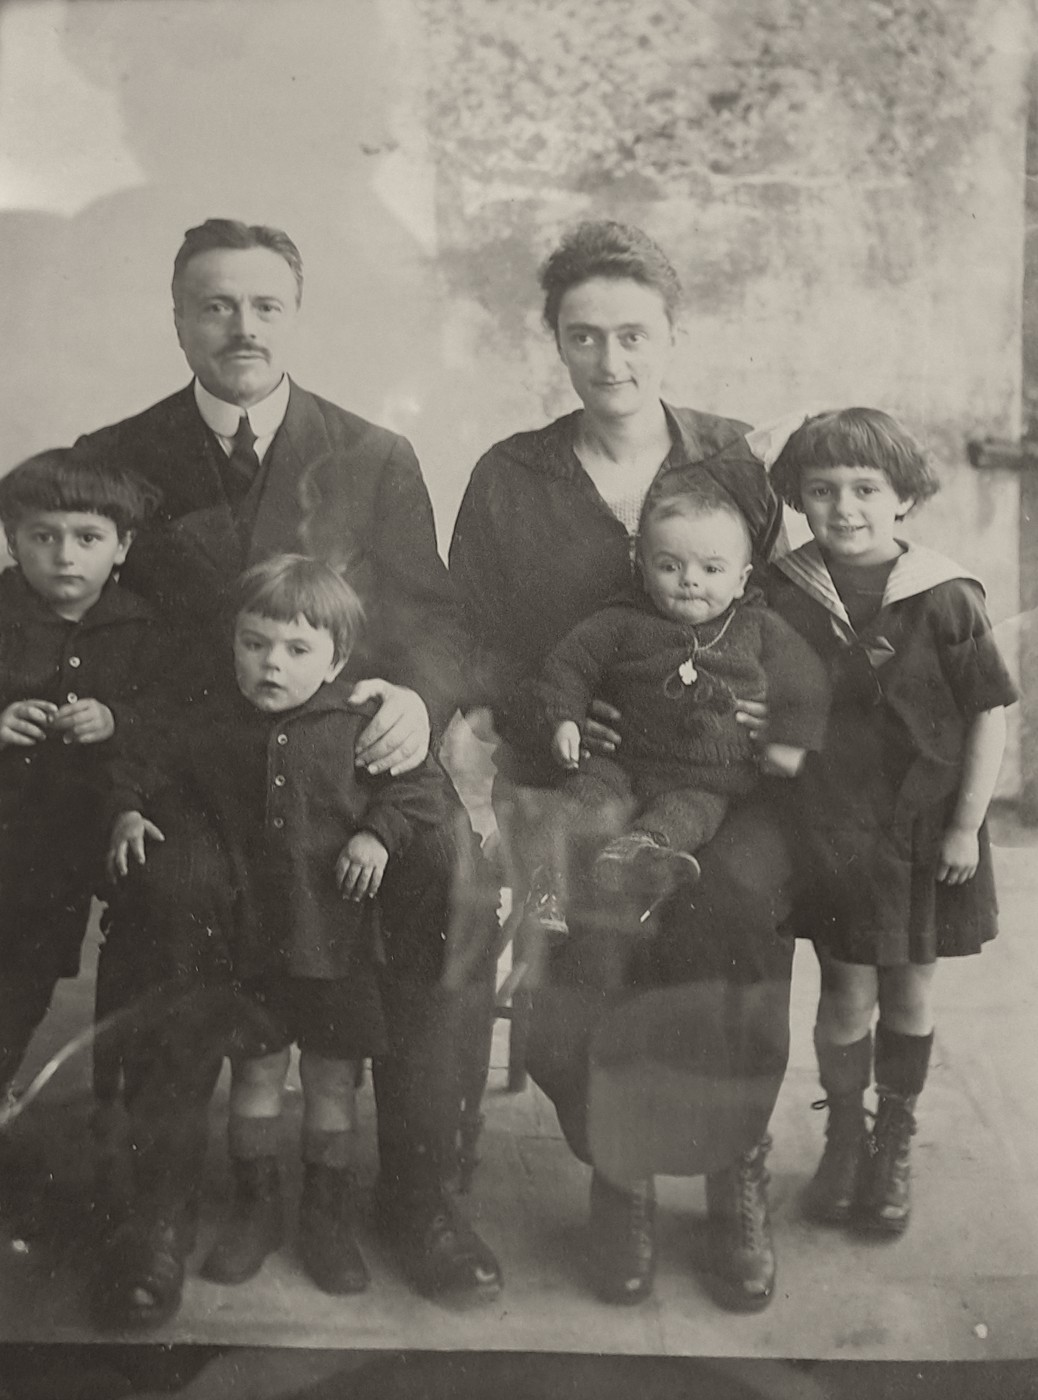
\includegraphics[width=0.48\textwidth,height=0.36\textheight,keepaspectratio]{illustrations/famille_combes_1925.jpg}\hfill
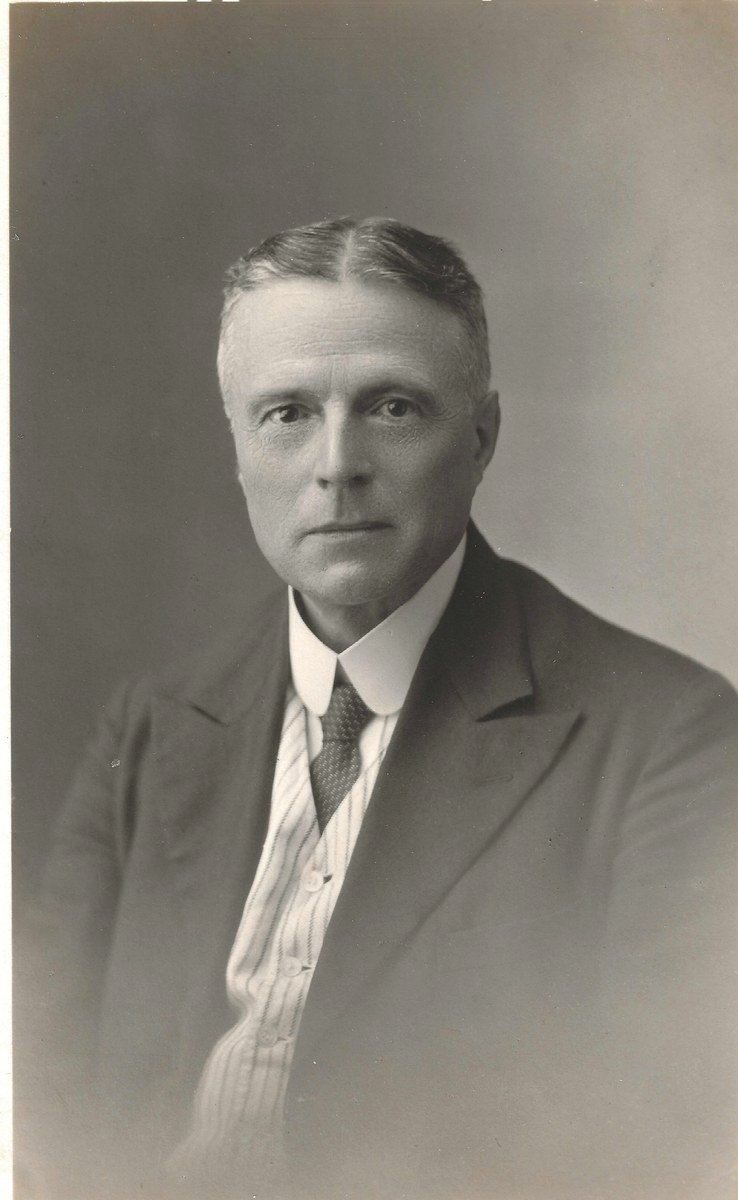
\includegraphics[width=0.48\textwidth,height=0.36\textheight,keepaspectratio]{illustrations/hippolyte_cambridge_1930.jpg}
\caption{À gauche, Hippolyte et Marguerite Combes et quatre de leurs enfants, milieu des années 1920 ; à droite, Hippolyte Combes à Cambridge, années 1930 (archives familiales).}
\end{figure}


À la rentrée de 1919, Hippolyte Combes fut nommé «~chargé de cours d'anglais (5\textsuperscript{e}~classe)~» au lycée de Montauban ; en janvier 1920, il habitait 55, rue du Moustier\footnote{\textit{Les Langues modernes}, \textit{loc.~cit.} ; fiche matricule ; «~Annuaire de l'Association pour 1921~», \textit{Les Langues modernes}, 19\textsuperscript{e}~année, 1921, p.~339.}. Il enseigna au lycée Ingres jusqu'en 1937. Après Valentine vinrent François (1920), Joseph (1921), Jean (1923), Marie-Thérèse (1925), Pierre (1928) et Michel (1930) (fig.~\ref{arbre-combes}). Trois naquirent à Saint-Chély-d'Apcher, en Lozère, dans la maison du docteur Fernand Vincens, mari de Madeleine Calmels, où la famille passait tous ses étés\footnote{P.~Combes, «~Mon grand-père~», et \textit{Étude} ; dates et lieux de naissance des sept enfants contrôlés dans le fichier des décès de l'INSEE.}.

Membre de l'Académie de Montauban à partir du 7~juin 1920, il fut «~très assidu aux séances~». Il y lut le 4~janvier 1932 «~Un “Poilu” de la Révolution : le sergent Landou de Montauban~», l'histoire d'un soldat parti illettré qui «~apprendra à lire entre deux combats~»\footnote{\textit{Recueil de l'Académie de Montauban}, année 1932, p.~47–57 ; éloge par H.~Pouvillon, \textit{loc.~cit.}, p.~150.}. Le 13~juillet 1928, dans le discours de la distribution des prix, il avait parlé aux élèves «~de la petite patrie et de nos amis les Anglais~», de l'occupation anglaise de Montauban (1361–1369) au passage de Wellington en 1814, d'après ses «~recherches passionnantes~» aux archives municipales ; il proposait des fêtes annuelles de la délivrance où les Anglais seraient représentés\footnote{\textit{Lycée Ingres. Distribution des prix du 13~juillet 1928. Discours prononcé par M.~Hippolyte Combes, professeur d'anglais}, brochure dédicacée à son fils Jean, archives familiales (couverture et p.~3–9).}.

En 1937, il obtint sa mutation au lycée de garçons de Toulouse. L'éloge de son successeur à l'Académie le dit «~aimé de ses élèves qui appréciaient sa méthode d'enseignement, son indulgence et sa bonté~», père de «~7 enfants admirablement élevés~»\footnote{H.~Pouvillon, \textit{loc.~cit.}, p.~150–151 ; voir aussi le discours du président Caldesaigues, \textit{ibid.}, p.~147. La tradition hésite entre 1937 et 1938 ; en février 1938, l'Académie tient le départ pour accompli : 1937 est le plus probable.}. Retraité en 1939, il enseigna l'anglais jusqu'en 1960 au Caousou, le collège des jésuites de Toulouse, dont il fut aussi, selon la tradition, le «~directeur civil~» et, de 1947 à 1966, le directeur pédagogique\footnote{P.~Combes, \textit{Étude} ; deux lettres de 1949 et de 1961 sont écrites sur papier à en-tête du Caousou (archives familiales).}. «~Professeur honoraire au Lycée de Toulouse~», il donna le 15~mai 1941, à l'hôtel d'Assézat, une conférence avec projections sur «~La Bête du Gévaudan~», sujet déjà traité à Montauban\footnote{\textit{Bulletin de la Société de géographie de Toulouse}, 1\textsuperscript{er}~avril 1941 (\url{https://rosalis.bibliotheque.toulouse.fr/ark:/12148/bpt6k6282699q}) ; \textit{Le Midi socialiste}, 13~mai 1941, p.~2 ; P.~Combes, \textit{Étude}.}. Il habitait 38, rue du Taur, la rue de ses parents en 1896\footnote{Lettre du 17~septembre 1949, archives familiales ; P.~Combes, \textit{Étude}.}. En 1964, à quatre-vingt-sept ou quatre-vingt-huit ans, il se disait encore très actif : le Caousou, des leçons particulières, de nombreuses conférences\footnote{P.~Combes, \textit{Étude}, qui résume cette lettre.}.

\subsection{La fin à Saint-Chély-d'Apcher}

Selon son petit-fils, ses conférences sur la Bête du Gévaudan commençaient ainsi : «~Dans la pittoresque Lozère où je reviens tous les ans~». À Saint-Chély-d'Apcher, le docteur Gabriel («~Gaby~») Vincens avait succédé à son père, le docteur Fernand Vincens\footnote{Courriel de Jacques Vincens, petit-fils d'Hippolyte Combes (fils de Paul Vincens et de Marie-Thérèse Combes), 18~octobre 2026. Il rappelle la formule favorite de «~Bon Papa~» dans ses lettres : «~Avec toute mon affection~». L'arbre de la branche Vincens doit beaucoup, selon lui, aux recherches d'une fille du docteur Gaby Vincens (Nicole) ; Pierre Combes a établi ceux des branches Combes et Calmels pendant ses séjours en Chine.}, et Hippolyte Combes y revint chaque été jusqu'à la fin. Il y mourut le 2~septembre 1970, d'une crise d'urémie, à l'Hôtel du Centre selon la famille ; il avait gardé «~jusqu'au bout~», écrit Pierre Combes, «~des facultés intellectuelles étonnantes~». Il fut inhumé dans le caveau familial de Millau, où Marguerite, morte à Millau le 19~mars 1974, le rejoignit\footnote{P.~Combes, \textit{Étude}, qui ne nomme pas l'hôtel (indication de la famille recueillie par l'éditeur) ; arbres de 2020 ; fichier de l'INSEE pour Marguerite Calmels. Le décès d'Hippolyte Combes manque au fichier de l'INSEE, lacunaire pour 1970 ; l'acte n'a pas été consulté.}. Il aurait tenu un journal jusque dans les années 1960, mais beaucoup de ses papiers furent détruits quand on vida l'appartement de la rue du Taur\footnote{P.~Combes, \textit{Étude}, qui mentionne un chapitre de ce journal sur «~une noce dans le Levezou~» (1963).}.

\subsection{Le carnet, les \textit{Feuillets de Route} et leur transmission}\label{intro:transmission}

Le \textit{Livre-Journal} est l'un des rares écrits personnels d'Hippolyte Combes qui subsistent, mais non le seul de la guerre. Le carnet renvoie lui-même, pendant la permission de Millau de février 1917, à un «~Journal~», «~feuille speciale~» (f.~71~r\textsuperscript{o}) ; des minutes et copies de lettres de 1915–1916 subsistent sur des feuillets de carnets quadrillés. Surtout, cinq feuillets autographes donnent le plan d'un livre : \textit{Feuillets de Route — Souvenirs d'un Interprète auprès de l'armée britannique — Récits divers, Impressions et Croquis} (annexe, p.~\pageref{annexe:doc6}). Le feuillet de division (\textit{«~— Journal — | 1915 — | 1916 — | — Nouvelles —~»}) prévoit un journal des années 1915–1916 ; il fait penser à des notes antérieures au présent carnet, ouvert le 25~juillet 1916, sans prouver qu'un premier cahier ait été écrit. Hippolyte Combes voulait y joindre vingt-deux chapitres de récits et croquis (\textit{Varia} ou \textit{Nouvelles}), de Toulon, Rouen et les \textit{1\textsuperscript{st} Irish Guards} jusqu'aux cantonnements d'hiver en Picardie. Le carnet et ces feuillets ont été conservés chez son fils François (1920–2006), agrégé de physique et professeur à Toulouse. Maurice Combes, fils de François, les a transmis à Pierre Combes, petit-fils d'Hippolyte et fils de Joseph. Le carnet a été photographié le 26~novembre 2025 ; les \textit{Feuillets de Route} ont été communiqués en octobre 2026\footnote{Courriels de P.-A.~Hauseux (23~novembre 2025 et 22~octobre 2026) et de Pierre Combes (26~novembre 2025 et 22~octobre 2026) ; date des photographies.}.

\subsection{L'homme du carnet}

Dans les deux brouillons du premier chapitre des \textit{Feuillets de Route} (\textit{«~Pourquoi je me suis décidé à écrire ?~»}, annexe, p.~\pageref{annexe:doc6}), Hippolyte Combes dit pourquoi il écrit. Il avait «~l[on]gs dédaigné d'écrire~», par «~Indifférence ou paresse~» et «~conscience de [son] insuff\textsuperscript{ce} litt\textsuperscript{re}~». À quoi bon noter «~même les gros évént\textsuperscript{s} de ma vie d'interprète~» ? Le public lui importe peu, et «~Mes Parents~»~: «~je les ai perdus~». Mais il a «~atroc\textsuperscript{mt} souffert de [sa] solitude — Les interprètes sont 1 peu des exilés~» : hors du bridge et des «~expéditions amoureuses~», on se sent avec les officiers «~à cent lieues d'x [d'eux]~», sauf avec «~ceux qui ont bcp voyagé — et séjourné lgs sur le continent~». Seul dans son «~billet (ma chambre)~», dans l'«~exist\textsuperscript{ce} ent\textsuperscript{t} monotone~» de l'hiver, loin des jeux auxquels «~les E[nglish] consacrent de longues heures~», il éprouve «~Le besoin, de + en + pressant, de m'extérioriser, de fixer qq pensées pour moi seul~». Il en restera «~des pages écrites au gré de ma fantaisie, simpl\textsuperscript{t}, car je hais tt ce qui a des prétentions litt\textsuperscript{res} — scènes vécues, croquis~» ; autour de lui «~vivent des êtres, des F[rançais] [paysans], des E[nglish] — je v\textsuperscript{x} les observer, et les comprendre — visage si banal q[u]'il soit est 1 livre qu'on peut lire facil\textsuperscript{t}~».

Le \textit{Livre-Journal} applique ce programme. Il est à la fois journal intime et livre de comptes : presque chaque journée se termine par le relevé des dépenses, au centime près. Hippolyte Combes y est un homme d'ordre, qui prend, dans son appartement de Toulouse, «~un plaisir extrême à regarder \& ranger~» ses affaires (f.~28~r\textsuperscript{o}). Il regarde les ciels, les arbres, les clochers, et achète des cartes postales presque partout où il passe : le carnet note une cinquantaine d'achats. Il relève les inscriptions des églises, examine les faïences et les médailles d'un vieux collectionneur de Raincheval (f.~22~v\textsuperscript{o}), rend visite à un couple d'instituteurs du Mesnil dont le fils est élève de l'École normale supérieure (f.~84~r\textsuperscript{o}). Dès les premières pages, le paysage dit son humeur : «~Melancolie éparse à travers atmosphère~» (f.~1~r\textsuperscript{o}) ; «~Silence et solitude funebre~» (f.~1~v\textsuperscript{o}). De son grenier, il écoute la prière du soir de ses hôtes (f.~5~v\textsuperscript{o}) ; il fait sonner une à une les cinq cloches de Montaudran (f.~29~r\textsuperscript{o}) et regarde la pleine lune de sa fenêtre (f.~38~r\textsuperscript{o}). L'abattement y a sa place --- «~Vie vegetative deprimante \& abrutissante~» (f.~15~v\textsuperscript{o}), «~Lis ou rumine. Triste vie.~» (f.~51~v\textsuperscript{o}), «~ces villages où vecu \LJinc{jadis} bien vide \& triste~» (f.~76~v\textsuperscript{o}), «~Impressions de solitude \& détresse morale~» (f.~79~r\textsuperscript{o}) ---, le calme aussi : «~Retrouvé parfaite sante morale~» (f.~78~r\textsuperscript{o}). Les départs lui coûtent, de Steenwerck (f.~13~v\textsuperscript{o}) comme d'Hérissart, qu'il croit quitter en mars 1917 (f.~82~v\textsuperscript{o}). En permission, il pense à ses morts. Près de Toulouse, il croit «~revoir mère et \LJinc{sœurs}, m attendant, cme autrefoi, gare~» (f.~66~r\textsuperscript{o}) ; à Millau, la première nuit, «~Pensé à Papa, Maman, Sœurs --- que j'ai tant aimés~», et il sanglote (f.~70~v\textsuperscript{o}). Le 1\textsuperscript{er}~février 1917, il se dit «~complèt\textsuperscript{t} détaché de Toulouse~» et prêt à la quitter «~pour n'y retourner jamais plus~» (f.~68~v\textsuperscript{o}) ; le lendemain, il regrette déjà son appartement «~rempli de souvenirs~» (f.~69~r\textsuperscript{o}). Il s'installera pourtant à Toulouse en 1937 pour le reste de sa vie.

Dans le carnet, la religion est discrète. Les églises sont des monuments et des abris, où il entre pour se reposer ou, comme à Doullens, pour rêver «~à mon aise~» (ff.~13~v\textsuperscript{o} et 33~v\textsuperscript{o}). Il y trouve une «~relique d St~Hippte, mon patron~» (f.~13~v\textsuperscript{o}), relève à Saint-Pol la nuit de prière de Benoît Labre (f.~16~v\textsuperscript{o}), achète un chapelet et deux images de sainte Thérèse (ff.~30~r\textsuperscript{o} et 32~r\textsuperscript{o}). À Toulouse, il entend la messe à Saint-Étienne avec Marguerite (ff.~29~v\textsuperscript{o} et 30~v\textsuperscript{o}), et les fiancés échangent leurs serments devant des tombes de religieux. Au front, il reste plutôt au seuil. Un dimanche de juillet 1916, il note l'église «~archi-comble~» de Saint-Jans-Cappel, puis s'assied presque en face, sur un petit pont, pour lire (f.~3~v\textsuperscript{o}). Il assiste à un office méthodiste britannique («~Wesleyans~», f.~22~v\textsuperscript{o}), sujet d'un chapitre prévu des \textit{Feuillets de Route} (\textit{«~XIX - Sunday service in village church~»}) ; il a aussi copié un poème wesleyen (annexe, p.~\pageref{annexe:doc4}). À la Toussaint, il visite le cimetière dévasté d'Albert et va le soir à un «~Church meeting~» (f.~45~r\textsuperscript{o}). À Toutencourt, deux dimanches de 1917, il entre à l'église pendant l'office et écoute le prône (ff.~78~r\textsuperscript{o} et 85~r\textsuperscript{o}). Le carnet ne mentionne de messe ni à Noël 1916, dont l'après-midi se passe au concert du foyer de l'Y.M.C.A. (f.~57~r\textsuperscript{o}), ni à Pâques 1917, consacré aux affaires (f.~89~r\textsuperscript{o}) ; à Millau, Marguerite va à la messe sans lui, et il monte rêver dans sa chambre (f.~70~v\textsuperscript{o}). Le carnet se situe entre l'étudiant «~alors agnostique~» de la tradition et le père de famille qui allait chaque dimanche, avec toute sa maison, à la messe de la cathédrale de Montauban\footnote{Courriel de Pierre Combes, 11~octobre 2021, archives familiales.}, avant de diriger les études du Caousou. La religion y est surtout liée au souvenir des siens.

Sur les Britanniques, il n'est ni anglophile sans réserve ni hostile. Il apprécie le mess de la 152nd Company, où il est admis en septembre 1916 (voir p.~\pageref{intro:mess}) : «~\LJinc{convers\textsuperscript{n}} anglais \& sorte de club où me retirer pour lire revues \& journaux~» (f.~21~v\textsuperscript{o}). Détaché à Acheux, il regrette sa compagnie (voir p.~\pageref{intro:detache}). Il lit un \textit{English novel} (f.~79~v\textsuperscript{o}), parle longuement de l'Australie avec le lieutenant Wentworth (f.~88~v\textsuperscript{o}), apprécie un sous-lieutenant de Jersey, «~très instruit et poète~» (f.~89~v\textsuperscript{o}). Mais il supporte mal certains officiers. Le lieutenant Curtis est «~ce crétin~», puis «~cet idiot~» (ff.~11~r\textsuperscript{o} et 15~v\textsuperscript{o}), et il part «~sans laisser de regret~» : «~A brainless ass~» (f.~53~v\textsuperscript{o}). Son successeur, un capitaine de vingt ans, ancien \textit{office boy} «~à 50~£ a year~», d'abord «~charmant~», devient vite «~présomptueux \& vain~» (ff.~53~r\textsuperscript{o}–v\textsuperscript{o} et 55~v\textsuperscript{o}). Le 24~décembre 1916\label{intro:bloody}, ce capitaine lance chez une habitante un «~Bloody France etc. !~» qui le blesse au point qu'il hésite «~à le reporter à French Mission~» ; le lendemain encore : «~Dois je faire 1~rapport à Mission fr\textsuperscript{se} ?~» ; après un second mot «~très regrettable~», une «~explication très calme, mais très ferme~» lui vaut les excuses de l'officier (ff.~56~v\textsuperscript{o}–58~v\textsuperscript{o}). En janvier 1917, il échange avec un autre interprète «~nos impressions \& jugements sur les English~» (f.~64~r\textsuperscript{o}), sujet des chapitres \textsc{xvi} à \textsc{xviii} prévus pour les \textit{Feuillets de Route} (\textit{«~Officiers anglais~»}, \textit{«~Mes officiers~»}, \textit{«~L'occupation angl\textsuperscript{se}~»}).

Dans le carnet, Marguerite est nommée une vingtaine de fois, de juillet 1916 à février 1917, avec des mots qui reviennent : «~Charmante de simplicité \& de tendresse confiante~» (f.~27~v\textsuperscript{o}), «~vraiment exquise de simplicité \& de charme~» (f.~66~v\textsuperscript{o}). Il l'appelle «~ma Femme~» plus d'un an avant les noces ; le mot de mariage n'apparaît pas. Le ton reste retenu, à la différence de la lettre de juin 1916, où il traitait de «~tas de blagues~» les «~abstractions~» de gloire et d'honneur --- «~Vivre avant tout~» --- et priait sa sœur de brûler le feuillet\footnote{Lettre du 16~juin 1916, citée.}. Dans le \textit{Livre-Journal}, la critique de la guerre n'apparaît qu'une fois, le 25~août 1916 : des «~Réflexions amères~», en partie illisibles, sur l'État qui mobilise «~nos corps~» et prend encore «~notre intellige[nce], notre cœur~» (f.~14~v\textsuperscript{o}). Pour le reste, Hippolyte Combes s'y montre sensible et inquiet, vite abattu mais soucieux de se reprendre : «~Peu à peu, rasséréné \& pris dessus~», écrit-il à Noël (f.~57~r\textsuperscript{o}). C'est la règle qu'il donnera à sa femme en 1918 --- «~sois philosophe et attends sans fièvre les événements~» --- et dont il faisait encore, en 1964, le secret du bonheur\footnote{Carte à Marguerite Combes, Paris, 25~novembre 1918 ; même conseil le 2~décembre («~attends sans fièvre les événements que nous réserve demain~») ; P.~Combes, \textit{Étude}, qui résume la lettre de 1964 : «~le secret du bonheur est de se maintenir philosophe~».}.
